\chapter{Diseño experimental y resultados}
En este capítulo se explicarán las decisiones tomadas en cuanto al diseño del experimento, con el fin de alcanzar los objetivos previamente mencionados así como los resultados obtenidos de dicho experimento.
\section{Diseño experimental}
Una vez estudiados los \hyperref[subsec:metodos/control_baxter]{mecanismos de control del Baxter}, se procederá a extraer una base de datos del controlador por posición del robot Baxter, así como diseñar una red neuronal capaz de aprender de este controlador.

\subsection{Extracción de base de datos}
A fin de conseguir un controlador basado en el propio de Baxter, se ha de obtener una base de datos de movimientos de los cuales aprender. Esta base de datos consistirá en las posiciones, velocidades y torques registradas por el robot, así como de las órdenes enviadas sobre la posición y la ratio de velocidad deseadas.

Para ello, haremos uso de la \hyperref[subsubsec:metodos/pythonAPI]{interfaz para el lenguaje Python} que ofrece Baxter, así como de la herramienta \hyperref[subsec:metodos/rosbag]{\texttt{rosbag}}.
\subsubsection{Ejecución}
El espacio vectorial de las siete dimensiones formadas por cada una de las articulaciones del Baxter se muestreará de manera uniforme, a fin de obtener una base de datos representativa del controlador que estamos aprendiendo. Esto significa que, para cada movimiento, se elegirán siete posiciones objetivo (una por articulación) de acuerdo a una distribución uniforme sobre el rango de cada articulación. De igual manera se elegirá una ratio de velocidad objetivo con distribución uniforme entre 0 y 1. El tiempo máximo empleado para cada movimiento será de 15 segundos, ya que es tiempo suficiente para permitir el movimiento entre puntos distantes entre sí a una velocidad baja, y por lo tanto, para todos los movimientos.

\subsubsection{Tratamiento}
Una vez obtenida las distintas bases de datos, se preparan para la fase de entrenamiento y evaluación de la red neuronal.

\paragraph{Ficheros \texttt{.bag}}
El primer paso consiste en transformar la base de datos en tipos de datos que entienda el lenguaje de programación Python.

Los ficheros obtenidos con \texttt{rosbag} tienen la extensión \texttt{.bag}, y consisten en ficheros conteniendo mensajes sobre los que se iteran. De esta manera, iteramos sobre cada mensaje y leemos su contenido, que consiste en el tema del cual proviene el mensaje, una marca temporal de su recepción por \texttt{rosbag}, y del mensaje en sí mismo.

La marca temporal corresponde al tiempo del reloj interno del ordenador en el cual se recibe el mensaje. Dado que la conexión entre el robot y el ordenador se realiza por tcp/ip, este tiempo diferirá del de generación en el robot. Para paliar con este problema, \texttt{ROS} dispone una marca temporal dentro del cuerpo del mensaje con el instante de creación del mensaje en el robot (de acuerdo a su reloj interno), además de un número de secuencia para ordenar los mensajes en el ordenador.

\subparagraph{Error en frecuencia}
Gracias a esta información, se percibió un error en frecuencia entre el reloj del ordenador y el del robot. Esto significa que, a una frecuencia de generación de mensajes de 100 Hz, el ordenador generó 100 posiciones y velocidades deseadas por segundo (suponiendo que es el que tiene el reloj ajustado correctamente), mientras que el robot generó 99 posiciones, velocidades y torques actuales. Para solventar este problema, en primera instancia se representó gráficamente la diferencia de mensajes obtenidos por parte del ordenador y el robot en función del tiempo (figura \ref{fig:resultados/diferencia}).

\begin{figure}[]
	\centering
	\begin{subfigure}[b]{0.45\textwidth}
		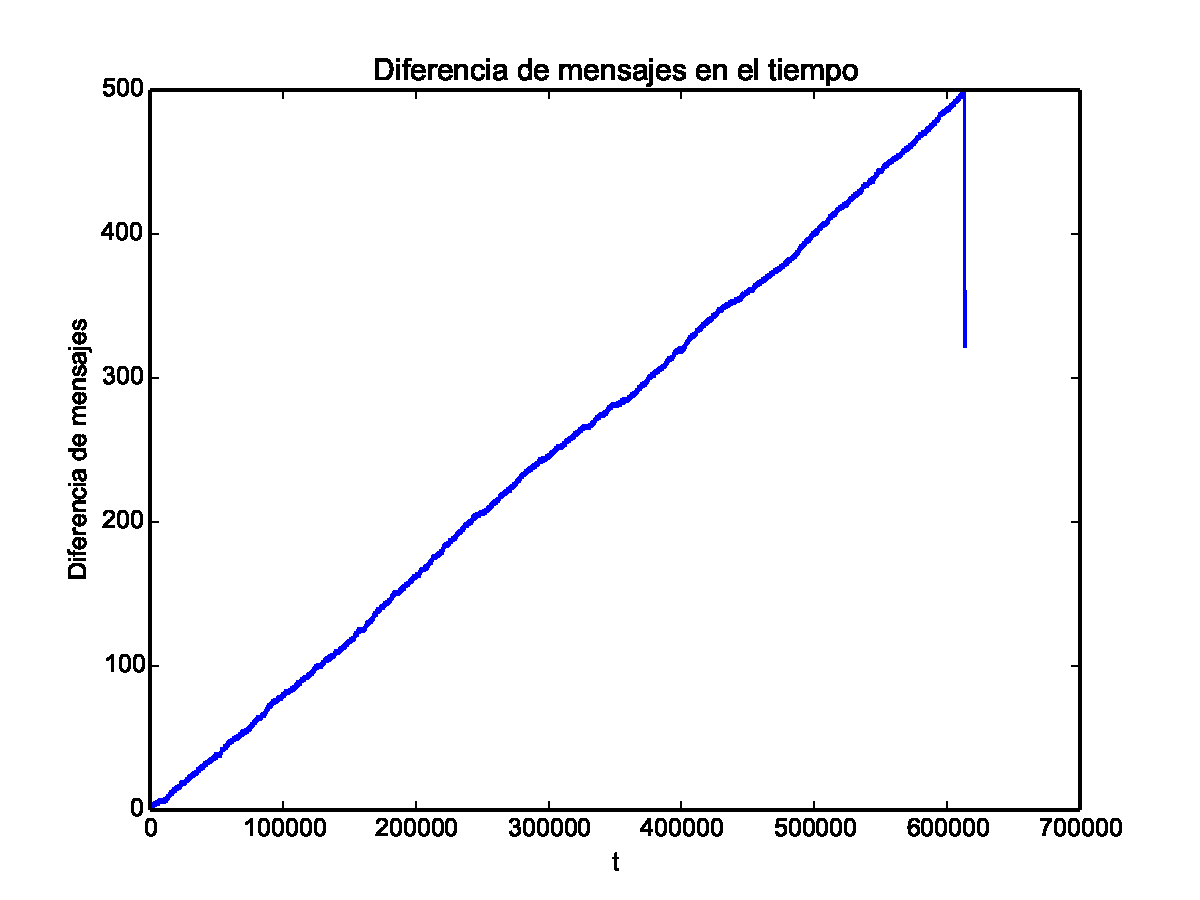
\includegraphics[width=\linewidth]{imagenes/resultados/diferencia.pdf}
		\caption{Señal sin procesar}
		\label{fig:resultados/diferencia}
	\end{subfigure}
	\begin{subfigure}[b]{0.45\textwidth}
		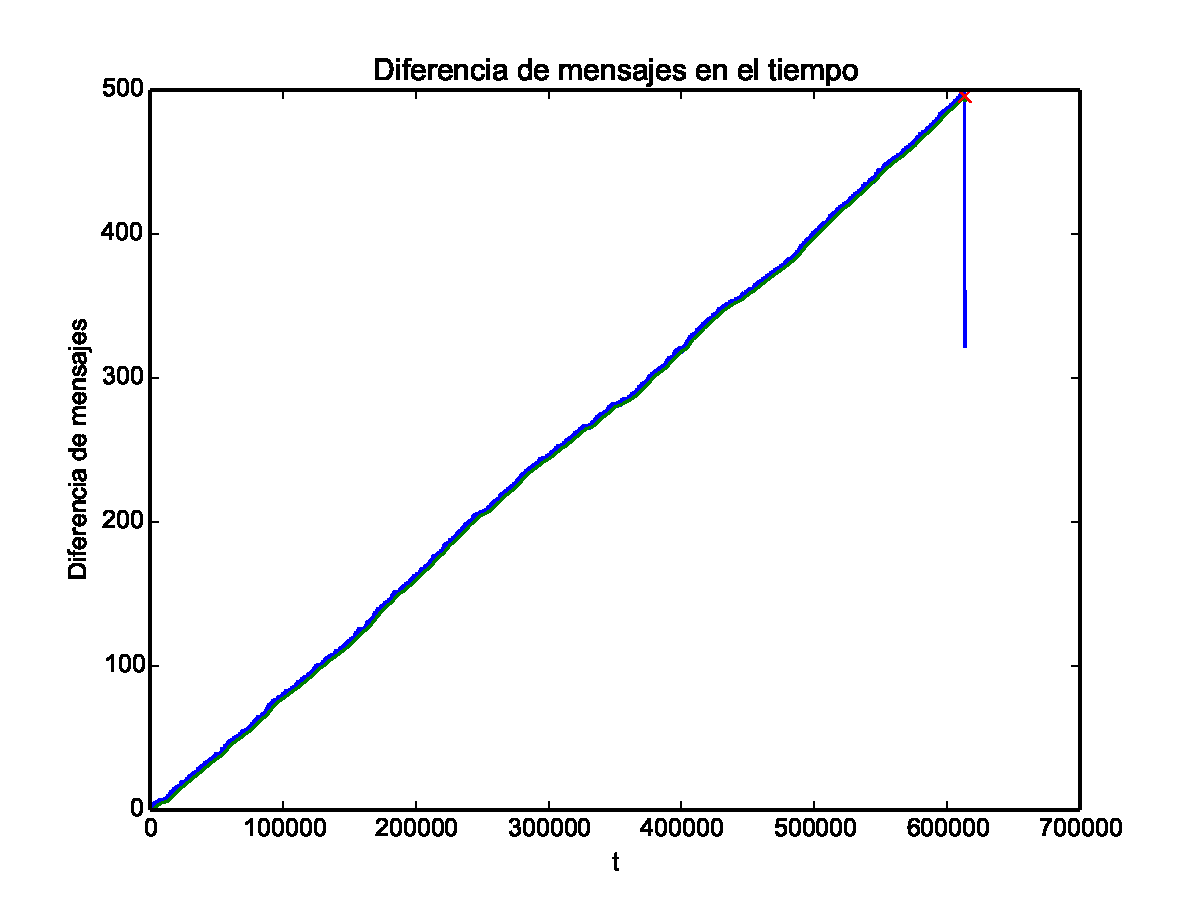
\includegraphics[width=\linewidth]{imagenes/resultados/diferenciafilt.pdf}
		\caption{Señal filtrada paso baja}
		\label{fig:resultados/diferenciafilt}
	\end{subfigure}
	\caption{Diferencia de mensajes recibidos del ordenador y del robot}
\end{figure}

Como se puede observar, esta diferencia crece con el tiempo, lo que significa que el ordenador genera mensajes a mayor velocidad que el robot. Es cuando el ordenador deja de generar mensajes cuando esta diferencia cae en picado, momento en el cual, los mensajes generados por el robot dejarán de corresponderse con las posiciones deseadas y pasarán a corresponderse con las posiciones, velocidades y torques del robot manteniendo la última posición alcanzada.

Por lo tanto, el objetivo será encontrar el momento en el que ocurre dicha bajada, es decir, el pico. El problema surge cuando la señal no es monótona, sino que, como se observa en la figura \ref{fig:resultados/diferenciadetalle}, crece y decrece en intervalos temporales pequeños (debido a la naturaleza a ráfagas de la señal). Para paliar con este inconveniente, se realiza un filtrado paso baja (con un filtro de media móvil) que elimine dicha componente frecuencial. El resultado es el que se observa en las figuras \ref{fig:resultados/diferenciafilt} y \ref{fig:resultados/diferenciadetallefilt}. A partir de esta señal, solo queda seleccionar el valor máximo de la misma. El valor obtenido es el número de mensaje recibido hasta el cual los mensajes son válidos.

\begin{figure}[]
	\centering
	\begin{subfigure}[b]{0.45\textwidth}
		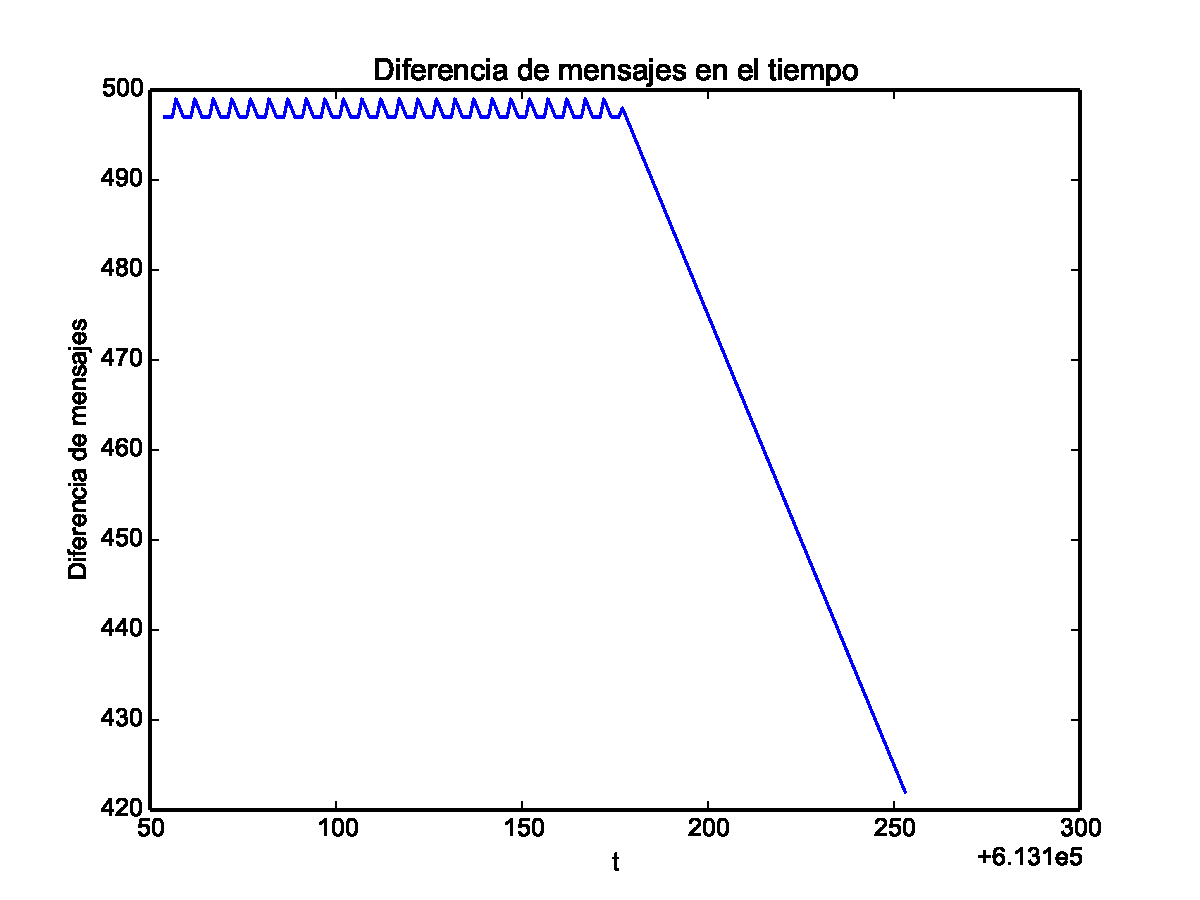
\includegraphics[width=\linewidth]{imagenes/resultados/diferenciadetalle.pdf}
		\caption{Señal sin procesar}
		\label{fig:resultados/diferenciadetalle}
	\end{subfigure}
	\begin{subfigure}[b]{0.45\textwidth}
		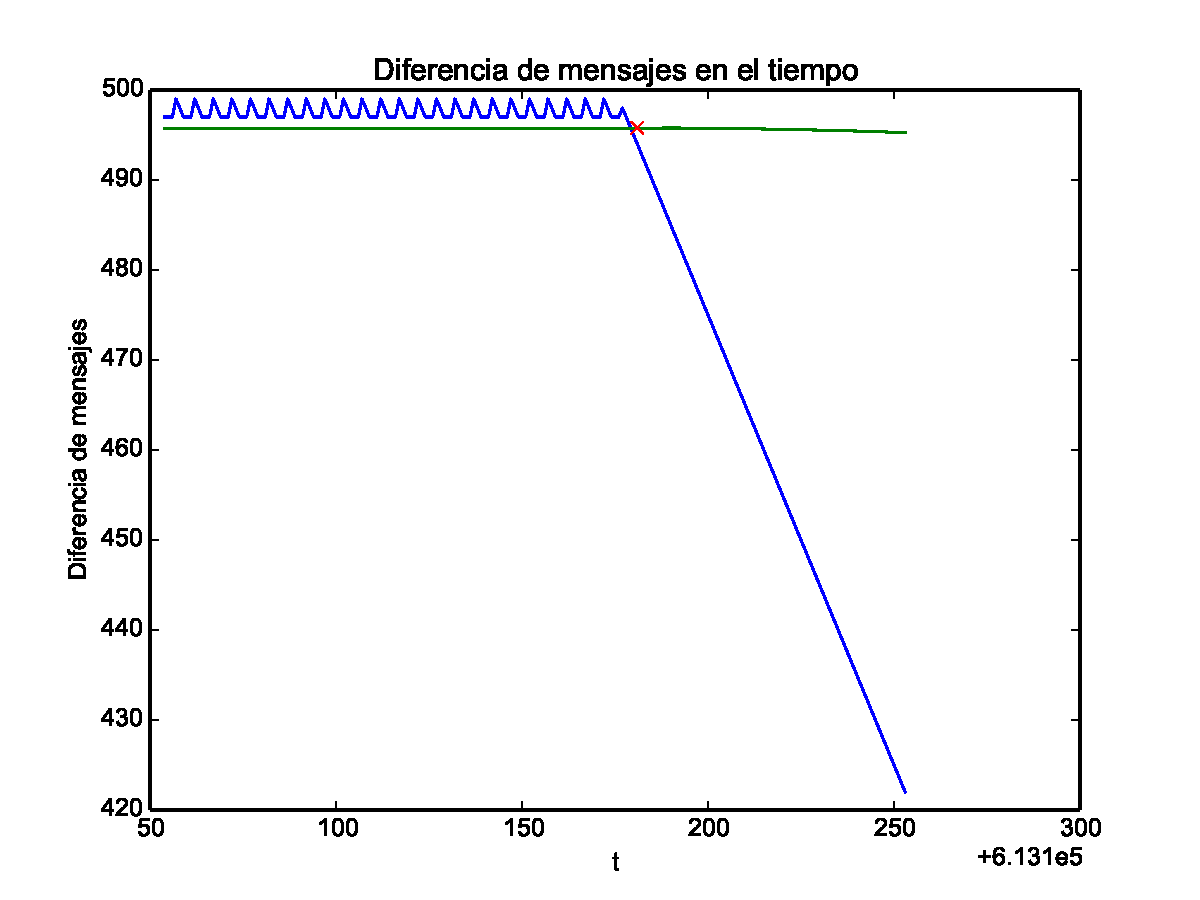
\includegraphics[width=\linewidth]{imagenes/resultados/diferenciafiltdetalle.pdf}
		\caption{Señal filtrada paso baja}
		\label{fig:resultados/diferenciadetallefilt}
	\end{subfigure}
	\caption{Detalle de diferencia de mensajes recibidos del ordenador y del robot}
\end{figure}

Dado que el control lo vamos a realizar desde el ordenador, adaptamos los mensajes recibidos al mismo. Esto lo hacemos mediante interpolación lineal en las posiciones, velocidades y torques recibidos.

De esta manera, se obtienen vectores de la misma longitud (en el tiempo) tanto enviados como recibidos.

\subparagraph{Ráfagas}
También se percibió la llegada a ráfagas en los mensajes provenientes del robot. Esto no supone un problema para preparar los datos, pero sí lo es a la hora de realizar un controlador realimentado que requiere la información que proporciona el robot sin desfases. El controlador propuesto en este trabajo no es realimentado, pero de serlo, una posible solución sería implementar el controlador en el propio robot (no ejecutarlo en el ordenador), aunque para ello habría que tomar nuevamente la base de datos o ajustarla a la frecuencia de generación de mensajes del robot. Otra posible solución consistiría en un predictor de posiciones y velocidades que ofrezcan al controlador esta información cuando no disponga de la misma. Por ejemplo, supongamos que en un instante concreto, llega una ráfaga de tres posiciones, velocidades y torques provenientes del robot. Esto significa que, dos instantes anteriores, el ordenador no ha obtenido ninguna información, por lo que la última posición, velocidad y torques conocidos son los obtenidos hace dos instantes temporales. En este caso, el predictor generaría 2 posiciones y velocidades (los torques serían la salida del sistema) para los instantes temporales que no disponen de información directa.


\subsection{Red Neuronal}
A continuación se estudia la viabilidad de la implementación de un controlador a partir del propio de Baxter basado en redes neuronales profundas.
\subsubsection{Viabilidad}
El primer problema a enfrentarse es el de demostrar que la red neuronal es capaz de aprender algo de los datos extraídos del controlador del Baxter. Por la capacidad de detectar colisiones sabemos que es un sistema realimentado, posiblemente con un controlador PID.

Se podría realizar un controlador donde el modelo dinámico (controlador anticipativo) fuera desempeñado por la red neuronal, y donde la realimentación fuera desempeñada por el controlador PID. También podría implementarse la realimentación como otra red neuronal, pero ambas aproximaciones tienen el problema de enfrentarse a la realimentación y al tiempo real (a una frecuencia de realimentación de 100Hz). Las redes neuronales profundas tienen el problema de ser pesadas en el cómputo (debido a las no linealidades usadas para la activación de las neuronas), poniendo en riesgo la capacidad de afrontar el problema en tiempo real.

Es por esto por lo que se decide hacer un controlador sin realimentación, donde los datos de entrada sean posiciones objetivo, posiciones en el momento de iniciar el movimiento, y velocidad objetivo, siendo los de salida una sucesión de torques a aplicar para alcanzar la posición deseada.

Para ello se elige una arquitectura basada en redes neuronales realimentadas, ya que las no realimentadas tienen la limitación de generar la misma salida ante la misma entrada, y siendo nuestra entrada única (debido a que el sistema no es realimentado), generaríamos siempre la misma salida, en vez de la sucesión de torques deseada.

Nos encontramos con el problema de, si el controlador implementado por Baxter es realimentado, ¿puede un modelo no realimentado aprender de este? % Quitar pregunta?
El controlador del Baxter tiene una estructura como la mostrada en la figura \ref{fig:desarrollo/feedforward_controller}. El funcionamiento es el siguiente:

\begin{enumerate}
\item El controlador realimentado genera una señal torque a partir de la realimentación de posición del sistema y la posición deseada.
\item El controlador anticipativo tiene en cuenta el modelo interno del robot y ajusta la señal de control generada por el controlador realimentado.
\item Se transmite la señal y el robot genera el torque enviado.
\item La aplicación genera una nueva posición que es recibido por los sensores y usado para la realimentación.
\end{enumerate}

\tikzstyle{block} = [draw, fill=blue!20, rectangle, 
    minimum height=3em, minimum width=6em]
\tikzstyle{sum} = [draw, fill=blue!20, circle, node distance=1cm]
\tikzstyle{input} = [coordinate]
\tikzstyle{output} = [coordinate]
\tikzstyle{pinstyle} = [pin edge={to-,thin,black}]
\begin{figure}[]
	\centering
	\deactivatequoting
	\begin{tikzpicture}[auto, node distance=2cm,>=latex']
	    % We start by placing the blocks
	    \node [input, name=input] {};
	    \node [sum, right of=input] (sum) {};
	    \node [block, right of=sum] (controller) {Controller};
	    \node [sum, right of=controller] (sum2) {};
	    \node [block, right of=sum2, pin={[pinstyle]above:Disturbances},
	          node distance=3cm] (system) {System};
	    % We draw an edge between the controller and system block to 
	    % calculate the coordinate u. We need it to place the measurement block. 
	    \draw [->] (sum2) -- node[name=u] {$u$} (system);
	    \node [output, right of=system] (output) {};
	    \node [block, below of=u] (measurements) {Measurements};
	
	    % Once the nodes are placed, connecting them is easy. 
	    \draw [draw,->] (input) -- node {$r$} (sum);
	    \draw [->] (sum) -- node {$e$} (controller);
 	    \draw [->] (controller) -- node {$e$} (sum2);
	    \draw [->] (system) -- node [name=y] {$y$}(output);
	    \draw [->] (y) |- (measurements);
	    \draw [->] (measurements) -| node[pos=0.99] {$-$} 
	        node [near end] {$y_m$} (sum);
	\end{tikzpicture}
	\caption{Sistema de control de Baxter}
	\label{fig:desarrollo/feedforward_controller}
	\activatequoting
\end{figure}

El controlador realimentado no es más que un sistema (lineal o no) que a ciertas entradas genera ciertas salidas (en función de su historia o no). El controlador anticipativo igualmente es un sistema que tiene en cuenta el modelo dinámico del robot, y por lo tanto los dos sistemas son reproducibles por una red neuronal. Por último, tenemos la realimentación, y es en este aspecto, donde la red neuronal tendrá que aprender a producir estimaciones de la salida provocada (posiciones de las articulaciones) al aplicar los torques.

Por lo tanto, la viabilidad de nuestro controlador depende de la capacidad de la red para generar dicha estimación de la realimentación.

Es por ello por lo que se utilizarán redes neuronales recurrentes, ya que tanto el controlador realimentado, como el anticipativo, como la realimentación en sí misma son sistemas que dependen de la historia de las señales de las que dependen, y esto es exactamente lo que hacen este tipo de redes.

\section{Resultados}
\subsection{Base de datos}
Por motivos de tiempo de entrenamiento, así como para aislar potenciales problemas a la hora de realizar el entrenamiento, se han tomado distintas bases de datos.

\begin{itemize}
\item [Todas las articulaciones] El grueso de nuestra base de datos se ha realizado a partir del movimiento de todas las articulaciones, a distintas velocidades, con un tiempo de espera de 15 segundos.
\item [Una articulación] Se ha aislado el problema del tamaño del espacio a muestrear (las siete articulaciones, cada una con su rango de movimiento) reduciéndolo a una de las siete articulaciones en todo su rango de movimiento. El resto de las articulaciones se mantienen quietas en la posición cero.
\item [5 segundos] En lugar de limitar el tiempo para cada movimiento a 15 segundos, se limita a 5 segundos, para así aislar el problema de desdoblar la red en un intervalo de tiempo tan alto 
($\SI{15}{\second} * \SI{100}{\hertz} = \SI{1500}{muestras}$).
\item [0.5 seg. ratio vel. 1] Es el caso más simple para entrenar la red. Se mueve una sola articulación (el resto se ubican en la posición 0) a máxima velocidad (relación de velocidad 1) durante 0.5 segundos. De esta manera obtenemos una base de datos muy amplia (más de 120 posiciones objetivo por minuto) con el problema del tamaño del espacio y del desdoblamiento temporal muy limitados.
\end{itemize}

Adicionalmente, se ha obtenido un conjunto de datos con combinaciones de distintas articulaciones, así como del brazo con las pinzas anexas para un tiempo máximo de 15 segundos y velocidad variable.